\chapter{Grafische Darstellung von Daten -- die MatPlotLib}
\label{chp:Matplotlib}
\epigraph{
	Real life seems to have no plots.
}{Ivy Compton-Burnett}

Menschen sind unheimlich gut darin, Bilder zu interpretieren. Computer haben ihre Stärke in der Auswertung von rohen Zahlen. Um nun die Früchte unserer Datenverarbeitung mit Python zu ernten, wollen wir Daten als graphische Plots ausgeben. Ein einfach zu bedienendes Mittel hierzu ist die MatPlotLib bzw. das Untermodul PyPlot. Das Modul MatPlotLib bietet tatsächlich so viele Funktionen, dass damit ein eigenständiger Kurs gefüllt werden könnte. Hier soll Ihnen eine Basis gezeigt werden, mit der Sie die häufigsten Aufgaben lösen können, und auf der Sie im Selbststudium leicht aufbauen können.

\section{Grundlagen}
An dieser Stelle möchte ich Ihnen zuerst einen einfachen Code zeigen, und diesen dann Zeile für Zeile \enquote{entziffern}:

\begin{codebox}[Beispiel: Einfacher Plot, width=.55\linewidth, nobeforeafter, equal height group = grpXmpSimplePlot]
\begin{minted}[linenos]{python3}
import math
import matplotlib.pyplot as plt

N = 100
X = [(x - N/2) / 10 for x in range(N)]
Y = [math.sin(x) for x in X]

plt.plot(X, Y)
plt.show()
\end{minted}
\end{codebox}
%
\begin{tcolorbox}[title=Ausgabe: Einfacher Plot, width=.45\linewidth, nobeforeafter, equal height group = grpXmpSimplePlot]
	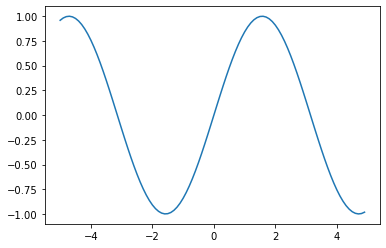
\includegraphics[width=\linewidth]{./gfx/plt-sin}
	\captionof{figure}{Einfacher Plot der matplotlib}
\end{tcolorbox}

In den Zeilen 1 und 2 laden wir Module -- zum einen das Modul \inPy{math}, mit dem wir die Daten generieren, die auf unserem Plot erscheinen sollen, und zum anderen die Matplotlib. Tatsächlich handelt es sich dabei um ein extrem umfangreiches Paket, weswegen wir nur einen Teil davon in unser Projekt integrieren: Das Untermodul \inPy{pyplot}\footnote{Die Matplotlib enthält Code zum Fenstermanagement, zur Interpolation von Kurven, Umgang mit Dateien, ... Alle diese Features bilden den Unterbau von \inPy{pyplot}, müssen aber nicht \enquote{offengelegt} werden, um für uns nützlich zu sein. Während \inPy{pyplot} intern alle diese Objekte und Funktionen benutzt und korrekt verwaltet, können wir uns auf das \emph{Interface} konzentrieren, das uns \inPy{pyplot} auf all diese Features bietet.}. Da dieser Modulname \inPy{matplotlib.pyplot} eher unhandlich ist, hat es sich eingebürgert, \inPy{plt} als Kurzname hierfür zu verwenden.

In den kommenden drei Zeilen generieren wir Werte, die schließlich geplottet werden sollen. \inPy{X} und \inPy{Y} sind jeweils Listen mit \inPy{N = 100} Elementen. Die Werte in \inPy{X} sind einfach gleichverteilte Werte im Abstand von \texttt{0.1}, rund um die \texttt{0} herum. Die Werte in \inPy{Y} enthalten jeweils den Sinus dieser \inPy{X}-Werte. Bis hierhin also haben wir noch nichts Neues gesehen.

In Zeile 8 wird nun die Funktion \inPy{plot} aus dem Modul \inPy{plt} aufgerufen. Diese Funktion bereitet alles vor, das nötig ist, um einen Plot zu generieren: Ein Arbeitsfenster, Achsen mit Beschriftung, Datenpunkte in den Graphen eintragen, ... All das wird aber nur im Arbeitsspeicher vorbereitet, jedoch noch nicht sichtbar gemacht. Grund hierfür ist, dass wir die Standard-Einstellungen noch abändern könnten. Wenn jede Änderung in Echtzeit umgesetzt würde, hätte dies ein unangenehmes Flackern auf dem Bildschirm zur Folge, bevor der Plot fertig aufgebaut ist. Stattdessen müssen wir manuell festlegen, wann unser Plot fertig beschrieben ist, \ie wann er auf dem Bildschirm erscheinen soll. Dies geschieht in Zeile 10

https://matplotlib.org/tutorials/introductory/pyplot.html


%https://matplotlib.org/api/pyplot_api.html


scatter, plot, bars, isosurface, subplots, post-edit, save files, hintbox on data usage, loglog, quiver

HISTOGRAMS